\section{Проектирование синхронного фреймворка}

Один из основных подходов, используемых при разработке платформы – это максимальная гибкость и расширяемость. В платформе используется абстракция – механизм, представляющая собой и на деле некий механизм, ответственный за определенную задачу синхронизации внутри платформы. При желании, разработчик, использующий платформу может для разных задач использовать готовые механизмы, но если считает, что они ему не подходят, то может добавлять свои механизмы, расширяя функционал платформы. В дальнейшем все вызовы будут обработаны в одном потоке, что исключает гонку за данные.

Продемонстрировать гибкость платформы можно наглядно на следующем примере: в платформе есть механизм, ответственный за запуск и исполнение всех модулей в системе; есть несколько вариантов этого механизма – обычный линейный, многопоточный, многопоточный с использованием пула потоков. При использовании системы на различных процессорах – одноядерных или многоядерных имеет смысл использовать различные режимы исполнения соответственно, чтобы исключить затраты на лишнюю синхронизацию и обеспечить максимальную производительность. Так, например, нет смысла запускать многопоточный режим на старом одноядерном процессоре, и в ту же очередь нет смысла не использовать возможность распараллеливания на многоядерных процессорах. Гибкость и расширяемость описываемой платформы позволяет подстроить ее под необходимую среду, в которой ей придется работать.

В данной работе под механизмами будет подразумеваться класс-обертка вокруг потоконебезопасного класса, которая инкапсулирует все вызовы к данному классу в функциональный объект и помещает его в потокобезопасную очередь. Использование механизма отложенных синхронизаций позволяет избавиться от проблем зацикливания при ситуации, например, когда какой-нибудь модуль отправляет сообщения сам себе. Также, позволяет с легкостью подобрать нужную реализацию очереди под конкретную ситуацию. 

Ниже представлена схема прототипа ядра разрабатываемой системы и базового набора модулей для робототехнической системы:

\begin{figure}[h]
    \centering{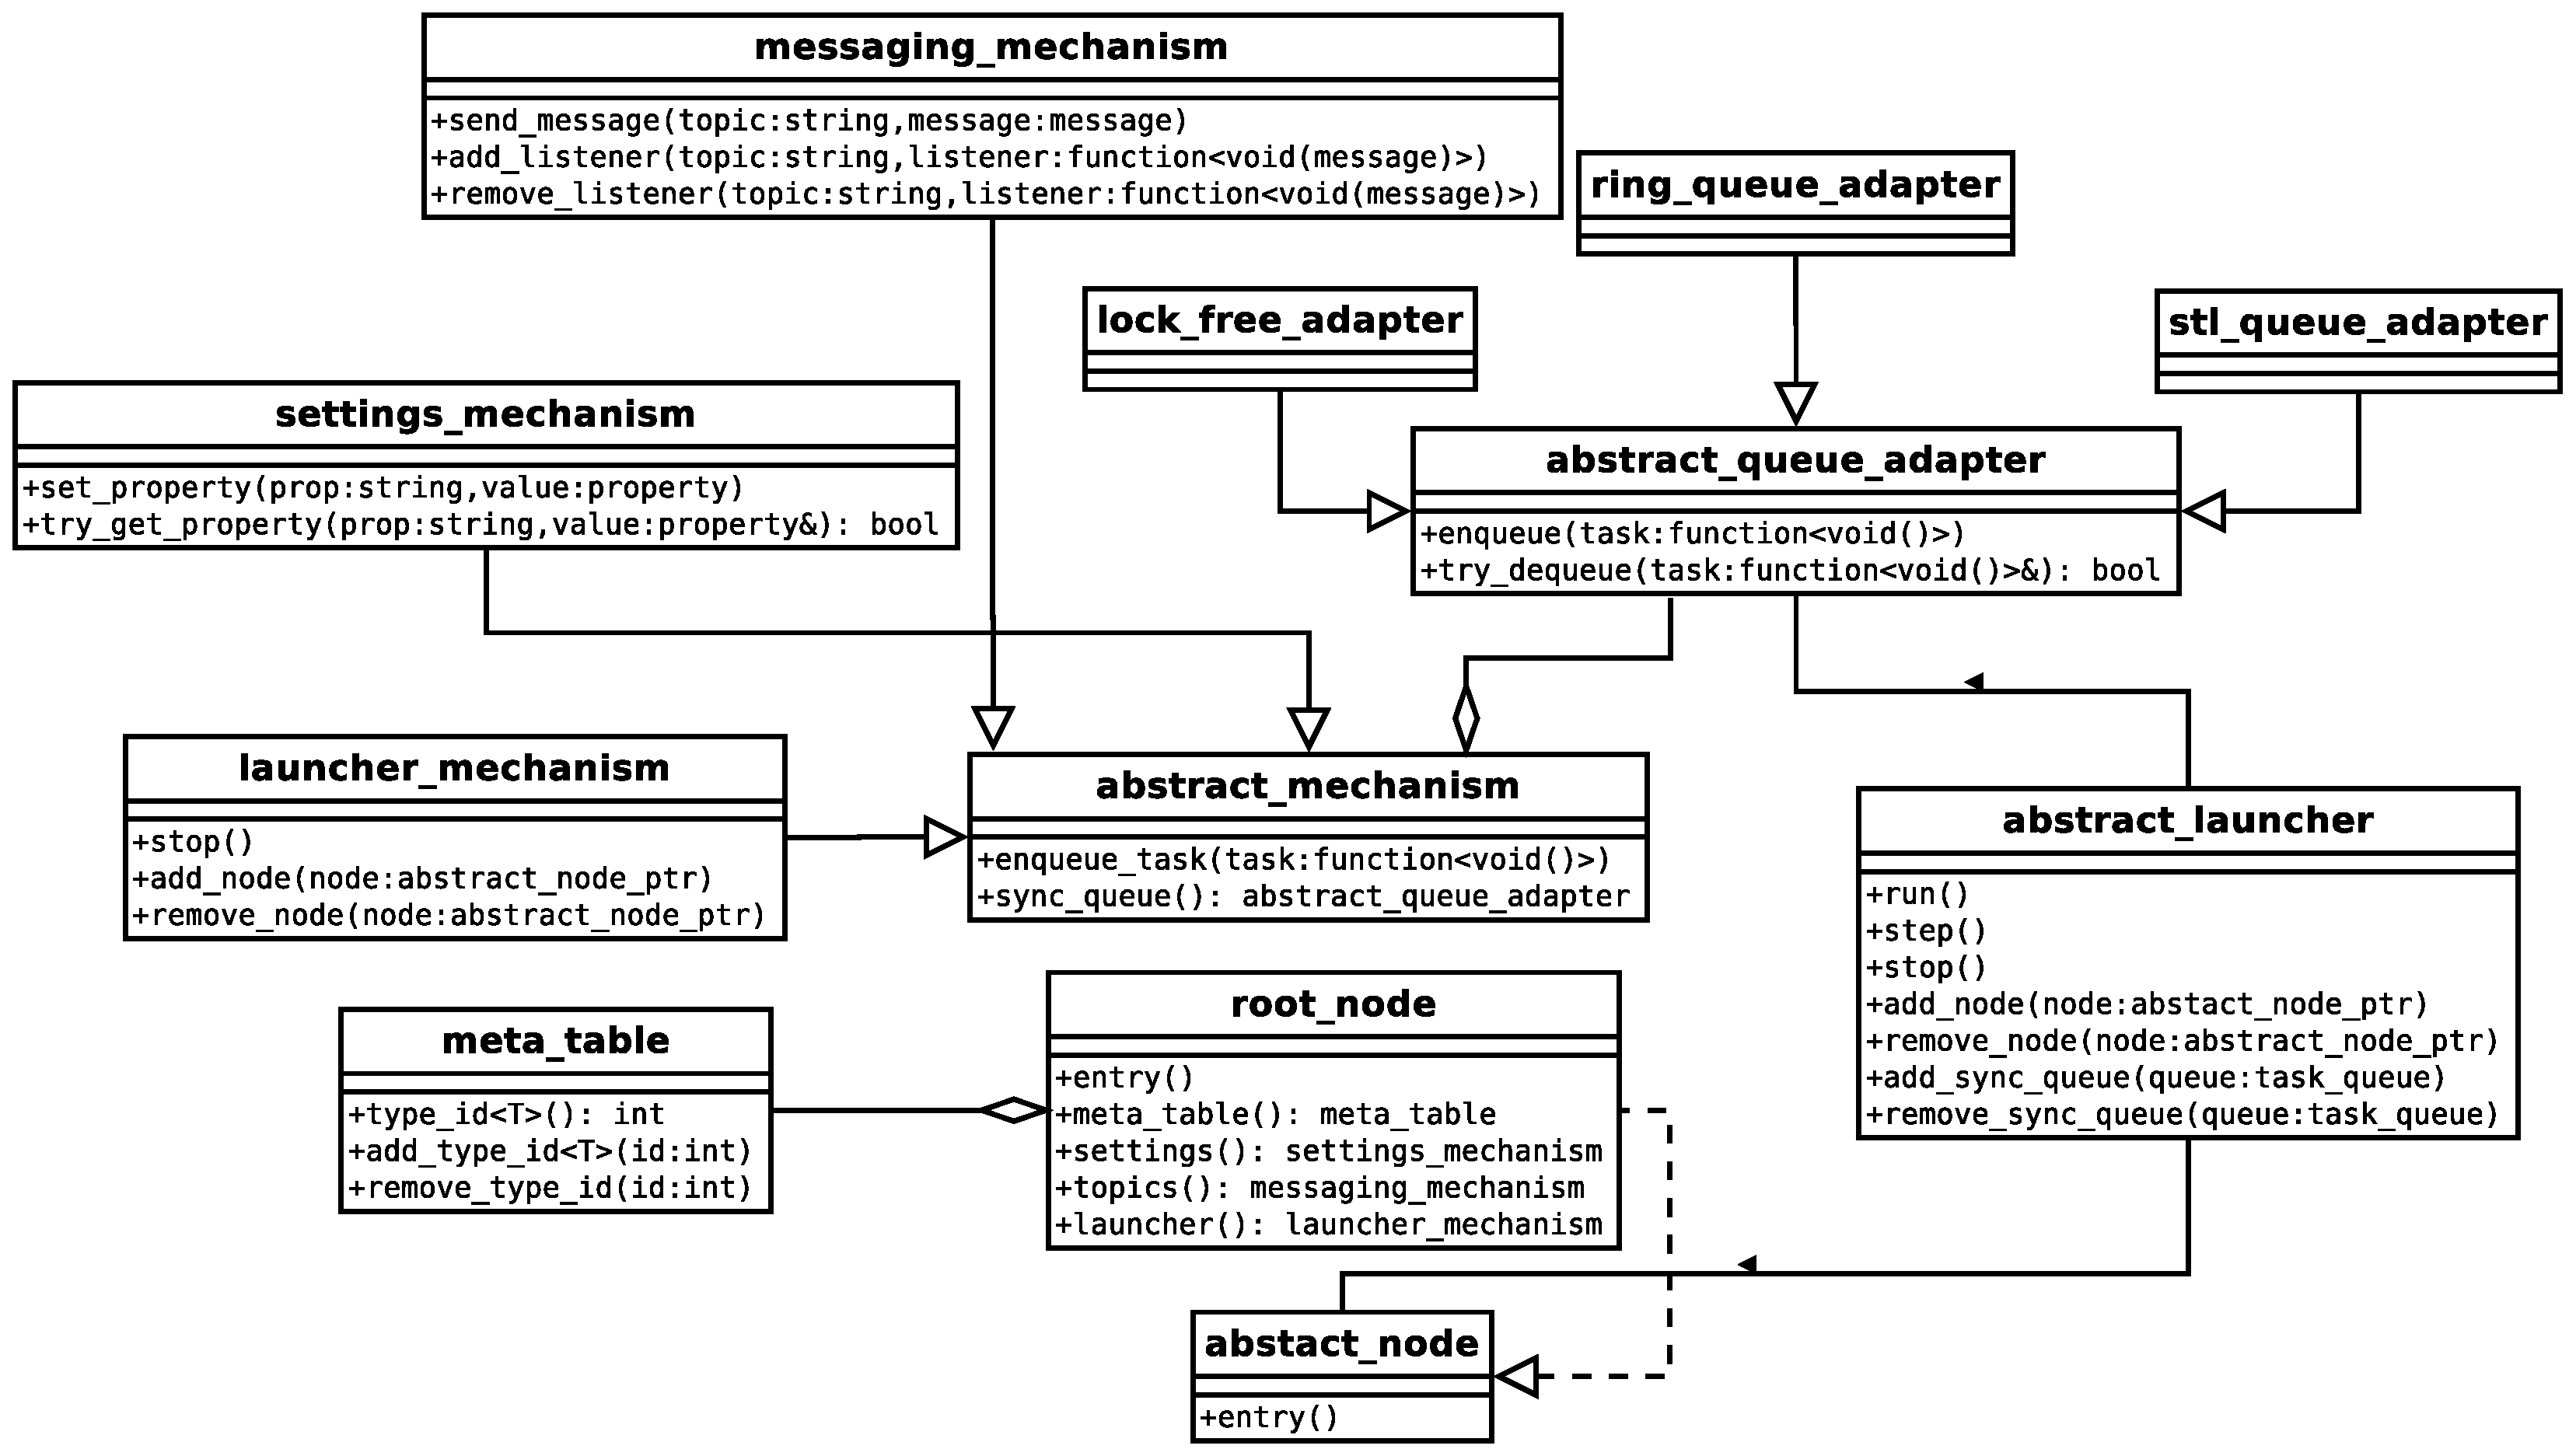
\includegraphics[width=1\linewidth]{2_2_1_sync}}
    \caption{Синхронное исполнение модулей в двух потоках}
    \label{im:2_2_1_sync}
\end{figure}

abstract\_queue\_adapter --- интерфейс компонента, необходимого для обеспечения отложенной синхронизации. Он передает все задачи по синхронизации на определенные очереди. Его возможные реализации:

stl\_queue\_adapter --- компонент, необходимый для работы с очередью из стандартной библиотеки c++ STL.

lock\_free\_adapter --- компонент, необходимый для работы с lock-free(без использования мъютексов) очередью. Используется реализация 

ring\_queue\_adapter --- компонент, необходимый для работы с  циклической очередью. 

abstract\_node --- интерфейс, позволяющий создавать независимые компоненты системы --- модули, каждый из которых может быть ответственнен за свой конкретный функционал. Модули не знают о существовании других модулей, то есть, они на самом деле, полностью независимы друг от друга. Из взаимодействие и исполнение обеспечено ядром системы. Такой подход к созданию этой абстракции также позволяет переиспользовать разработанные на ее основе модули при различных конфигурациях описываемой робототехнической платформы. 

abstract\_mechanism --- интерфейс компонентов системы, обеспечивающих какой-либо вид взаимодействия между модулями. Сама абстракция обеспечивает возможность версионирования конкретных механизмов.

launcher\_mechanism --- компонет, реализующий интерфейс abstract\_mechanism, обеспечивающий взаимодействий с конкретной реализацией AbstarctLauncher, позволяет добавлять и удалять модули, запускать и останавливать систему.

messaging\_mechanism --- компонет, реализующий интерфейс abstract\_mechanism, обеспечивающий возможность коммуникации и обмена данными между модулями путем отправки сообщений.

services\_mechanism --- компонет, реализующий интерфейс abstract\_mechanism, обеспечивающий возможность запуска требуемых методов по их имени.

В данной архитектуре сделан упор на расширяемость и возможность создания своих реализаций каждой из абстракций, что позволяет не только расширять функционал робототехнической платформы, но и гибко конфигурировать ее под конкретные нужды. Следует отметить, что представленное описание архитектуры не является полным и финальным. Некоторе из компонентов не представлены, некоторые находятся в стадии доработки. 

